%! Author = cspiller
%! Date = 16/11/2022

% Preamble
\documentclass[12pt, english]{article}

% Packages
% -- Typographic rules
\usepackage[english]{babel}
% -- Extended colors
\usepackage[dvipsnames]{xcolor}
% -- Embedded hyperlinks
\usepackage[colorlinks=true,linkcolor=BrickRed,citecolor=Fuchsia,pagebackref=true]{hyperref}
% -- Better text justification
\usepackage[nopatch=eqnum, auto=true, babel]{microtype}
% -- Images from file
\usepackage{graphicx}
% -- Better lists
\usepackage{enumitem}
% -- Bibliography format and access
\usepackage{natbib}
\usepackage{usebib}
% -- Glossary build
\usepackage[abbreviations]{glossaries-extra}
% -- Allow tables to cross pages
\usepackage{ltablex}
% -- Inline and display quotations
\usepackage[autostyle]{csquotes}
% -- Defines relative textsize commands
\usepackage{relsize}
% -- Used for AtBeginEnvironment hook
\usepackage{etoolbox}
% -- Adds extra symbols for quotations
\usepackage{textcomp}
% -- Adds better formatting for captions
\usepackage{caption}
% -- Visualise and change page layout
\usepackage{layout}
\usepackage{geometry}

% Setup table column sizes (big and small)
\newcolumntype{z}{X}
\newcolumntype{s}{>{\hsize=.5\hsize}X}
% Setup page geometry
\geometry{
    a4paper,
    total={165mm,252mm},
    left=25mm,
    top=25mm,
}
% Makes display quotation smaller
\AtBeginEnvironment{quotation}{\smaller}
% Path to store image files for use in the document
\graphicspath{ {images/} }
% Import bibliography file
\bibinput{main}
% Glossary setup
\loadglsentries{glossary.tex}
\makeglossaries

% Document
\begin{document}
%    Title Page
    %! Author = cspiller
%! Date = 17/11/2022

\newcommand{\reportversion}{Interim}

\begin{titlepage}
    \begin{center}
        \vspace*{1cm}

        \huge
        \textbf{Spatialisation As A Service (SaaS)}

        \vspace{0.5cm}

        \large
        \reportversion~Project Report

        \vspace{1.5cm}

        \LARGE
        \textbf{Callum John Spiller}

        \vspace{1.5cm}

        \small
        Programme of study:\\
        \textbf{BSc FT Computer Science (Apprenticeship)}

        \vspace{1cm}

        Supervisor:\\
        \textbf{Johann Pauwels}

        \vfill

        \footnotesize
        Final Year\\
        Undergraduate Project 2022/23

        \vspace{0.5cm}
        
\includegraphics[width=0.4\textwidth]{qmlogo}
        \vspace{0.5cm}

        School of Electronic Engineering and Computer Science\\
        \today

    \end{center}
\end{titlepage}
    \newpage

%    Abstract Page
%    \thispagestyle{plain}
\begin{center}
    \vspace{0.9cm}
    \textbf{Abstract}
\end{center}

Lorem ipsum dolor\ldots
%    \newpage

%    Contents
    \tableofcontents
    \newpage

%    Glossary
    \printglossaries

%    Main Content
    %! Author = cspiller
%! Date = 17/11/2022
\thispagestyle{plain}
\newpage
\section{Introduction}\label{sec:introduction}
\subsection{Project Background}\label{subsec:project-background}
\normalsize

This project has been undertaken as a part of a degree apprenticeship with~\gls{sie}.\
As such, the final year engineering project for this author will consider the business domain of the sponsoring company.\\

With the release of the~\gls{ps5} in November 2020,~\gls{spatial_audio} technology has come into focus for~\gls{sie} as game developers seek to leverage the~\gls{tempest_3d_audio} espoused by the video game console.
In addition,~\gls{sie} is undergoing a shift to cloud-based infrastructure\footnote{like many other companies relying on web technology~\citep{cc_overview}} across the wider business in order to leverage the cost, flexibility, and reliability benefits that cloud technology affords~\citep{cc_overview}.\\

With respect to these developments in the business, this project seeks to engage both of these emergent technologies in order to address one of~\gls{sie}\textquotesingle s major~\glspl{sla} with a software solution.\\

\subsection{Problem Statement}\label{subsec:problem-statement}

The onboarding of~\glspl{pspartner} to the developer and publisher platforms managed by~\gls{sie} has been a targeted area for improvement within the company.
The primary challenge the business has faced in this area has been the reduction of friction in the process of getting~\glspl{pspartner} into the PlayStation ecosystem.\\

While the~\gls{pspartner} onboarding process has been automated and refined over time, this author argues that the ability for potential~\glspl{pspartner} to engage with and trial PlayStation's spatial audio technology is too restricted.\\

This project is based upon the hypothesis that, for a user who wishes to experiment with or experience~\gls{spatial_audio}, the barrier for entry is too high.
Engaging with a working demonstration of customisable~\gls{spatial_audio} requires a user to perform a significant amount of preparation on a local machine;
it demands a time commitment and pre-requisite technical knowledge that is far greater than is reasonable for an interested party to quickly evaluate what is possible.\\

Currently~\glspl{pspartner} who want to experiment with~\gls{tempest_3d_audio} must apply and order a~\gls{ps5} development kit, wait for it to arrive, set it up, then figure out how to engage with the~\glspl{api} provided by~\gls{sie}\textquotesingle s~\gls{devnet}.
This process is time-consuming and not optimal for a~\gls{pspartner} who wishes to get a quick insight into what is possible.\\

This project proposes an alternative solution where a~\gls{pspartner} who wishes to engage with the~\gls{spatial_audio} paradigm is able to experiment using a familiar audio file of their choosing.
The fact that the system will be accessible through a browser will mean that the~\gls{pspartner} will have much easier access, increasing the overall positive impression of the~\gls{pspartner} platform.\\

\subsection{Project Aims}\label{subsec:aims}

The primary aim of this project is to research, design, and engineer a web service that allows a user to easily experience~\gls{spatial_audio} in a way that reacts to their input.\\

The proposed workflow would allow a user to use a standard web browser\footnote{The project will most likely be designed for interaction through Chromium-based browsers and Firefox} to upload an audio file to a webpage and then receive back a new audio file that has rendered the stems from the original file into a \textquotesingle spatialised\textquotesingle ~format informed by \glspl{hrtf}.
All the audio processing would execute in \gls{aws} cloud environments to circumvent any real-world hardware requirements and challenges.\\

For vital information security reasons, the prototype produced as a part of this project will not feature any proprietary~\gls{sie} software and instead use only libraries that exist in the public domain.
As such, this prototype can be considered a~\gls{poc} where, if successful,~\gls{sie} software might be transplanted into the serverless pipeline.

\subsection{Project Objectives}\label{subsec:project-objectives}

In order to achieve the aims set out in Section~\ref{subsec:aims} the project must produce a number of deliverables:

\begin{enumerate}
    \item A project plan which outlines the timeline of both the research and development of the project
    \item A review of pertinent literature relating primarily to:
    \begin{itemize}
        \item Audio spatialisation
        \item Web audio \glspl{api}
        \item Cloud infrastructure (including those available from \gls{aws})
    \end{itemize}
    \item A review of existing stereo-to-ambisonic services and technologies.
    \item A functioning stereo-to-ambisonic serverless pipeline.
    \item A frontend that enables a user to interact with the conversion pipeline by uploading and downloading audio files, as well as setting parameters for conversion through a web~\gls{api}.
    \item A testing framework that supports iterative development.
    \item A report on user testing, including feedback from stakeholders.
    \item A review and analysis of how the produced system has met or missed the targets.
\end{enumerate}

\subsection{Research Questions}\label{subsec:research-questions}

In order to guide the research and development process of the proposed system, this report will seek to answer the following research questions:

\begin{enumerate}
    \item How is spatial audio rendered?
    \item Who might be interested in experiencing spatial audio, how might they do it, and why?
    \item What are the existing ways in which spatial audio can be experienced, and how accessible are they?
    \item Starting with a standard music file, what is the best way to demonstrate the capabilities of spatial audio rendering?
    \item How can intensive audio processing be performed in cloud environments?
    \item How might audio that is rendered in the cloud be delivered efficiently back to a web front-end?

\end{enumerate}
    %! Author = cspiller
%! Date = 17/11/2022

\thispagestyle{plain}
\newpage
\section{Literature Review}\label{sec:literature-review}

\normalsize

As outlined in~\ref{subsec:aims}, this project attempts to engage with cloud infrastructure, spatial audio processing, and web development frameworks.
To approach these topics thoroughly, this report performs a review of pertinent literature.
In doing so, this report considers and incorporates existing ideas in these fields while providing a foundation from which to answer the research questions listed in~\ref{subsec:research-questions}.

\subsection{Cloud Computing}\label{subsec:cloud-computing}

Ever since internet service providers began the commercialisation of cloud computing, it has become one of the major trends in the technology space~\citep{cc_overview}.
According to~\citet{cc_overview}, `cloud computing' is one of the most vague terms when it comes to the description of the technology on account of the breadth of its application

% TODO Continue from here - explain cloud concepts and benefits, downsides and challenges

s2\citep{cc_challenges}

Cloud computing technology is dominated by three major players, each with their own style of cloud services:
\begin{enumerate}
    \item Amazon's Web Services which began as a means of server virtualization~\citep{awsintro}
    \item Google's Cloud Platform, described by~\citet{cc_overview} as a technique-specific sandbox that calls itself a~\gls{paas}~\citep{googlecloudintro}
    \item Microsoft's Azure Network~\citep{azurefundamentals}
\end{enumerate}

% TODO describe current state of public cloud landscape and current capabilities of these platforms and effect on businesses



\subsection{Audio Spatialisation}\label{subsec:audio-spatialisation}
\subsubsection{Origins}

\citet{blauert_spatial} notes in their seminal text,~\textit{\usebibentry{blauert_spatial}{title}}, that: \textquote{human beings are primarily visually-orientated}, and that the other senses are less developed in comparison.
This difference has been mirrored in the history of scientific research.
\citet{wade_binaural} note that research in binaural hearing was developed later than binocular vision partially due to the difficulty in controlling the audio stimuli in experiments.
It was only later on that the concept of distinction between the~\textit{sound event} and the~\textit{auditory event} as influenced by binaural hearing became prevalent.
\citet{blauert_spatial} explains that this distinction informs the practice of audio replication analogous to its originating sound event:

\begin{quotation}
    The telecommunications engineer, of course, is especially interested in just those cases in which the positions of the sound source, and the auditory event do not coincide.
    The telecommunications engineer seeks to reproduce the auditory events that occur at the point where a recording or transmission originates, using the smallest possible number of sound sources (e.g., loudspeakers)~\citep{blauert_spatial}.
\end{quotation}

The patent filed in 1958 by Alan Dower Blumlein\footnote{\citep{blumlein-patent}} details an early stereophonic system, which exploits the human sound localization ability for the enhancement of entertainment experiences\footnote{This author acknowledges that this is not the first example of this kind of system; the control of inter-aural time differences was pioneered by Cl\'ement Ader as early at 4 years after Bell's invention of the telephone. This was for the purpose of rendering a spatial transmission of the Paris Opera. This further solidifies a history of the desire for spatial immersion in entertainment.}~\footnote{There is a rich history of considering space in the composition of music in Western Classical tradition, with Italian renaissance composers writing for \textit{cori spezzati}, or multiple choirs that are spatially separated~\citep{spezzati}. This author mourns that the topic of spatialisation in historic acoustic performance goes beyond the scope of this report.}.
Blumlein observed that in film theatres there was a certain level of cognitive dissonance whereby the actor’s voices sounded like they were coming from a different location than where they appeared on the screen~\citep{alexander_blumlein}.
This patent, in response, specifically outlines methods for introducing stereophonic audio to sound film as a means of increasing the perceived~\textquote{quality} of the entertainment experience.
Blumlein acknowledges that human binaural hearing is responsible for the ability to localize sound, and his patent is an example of how one might induce an auditory event that exhibits spatialisation on the horizontal plane through the control of inter-aural time differences~\citep{blumlein-patent}.

The patent marked an improvement in the way that auditory events might be replicated by introducing this form of spatialisation, and the vestiges of Blumlein`s ideas can be observed in modern spatial audio techniques~\citep{spatial_techniques, beyer_acoustics}.
What is perhaps the most salient aspect of the document, however, is that it recognizes the physiological factors that are involved in human sound localization.
These physiological factors explored and expounded upon by~\citet{blauert_spatial}, and, as noted in the 1996 revision of his book, become more important as audio spatialisation and entertainment technology attempts to induce auditory events that imply three-dimensional audio spaces.

\subsubsection{From two to three}

\begin{quotation}
    The external ears superimpose linear distortions on the incoming signals, which, in each case, are specific for the direction of incidence of the sound wave and the source distance.
    In this way, spatial information is encoded into the signals that are received by the eardrums~\citep{blauert_spatial}.
\end{quotation}

\citet{roginska2017immersive} note that:~\textquote{the word `binaural' refers, at the most basic level, to hearing with two ears, but it later came to include all the spatial cues from the ears, head, and body of a listener}.
Binaural recordings can therefore refer to the practice of capturing sounds that incorporate human physiology.
This is executed with dummy mannikin heads with microphones placed inside the ears so that sound entering them are affected by the `blocking' nature of the head;
developments in this technology rapidly sped up throughout the 20th century~\citep{binaural_paul}.
While other forms of spatial representation were developed in this time period~\citep{gerzon_periphony, noisternig_ambisonic, wave_field}, technology that considers the physical and physiological factors in human listening when attempting to induce auditory events that feature sound localization.

\citet{roginska2017immersive} identify that while capturing binaural audio is relatively easy, realizing the same effect through post-recording production is considerably harder and poses the challenge of modelling the human spatialization facility.

\subsubsection{Getting the head in the game}

The~\glsaccessfirst{hrtf} can be described as a representation of the perceptual cues that facilitate human sound localization as a sound propagates from its source to the human ear~\citep{Suzuki2011}.
This modelling of the human sound localization facility allows for this~\gls{hrtf} to be applied to a sound before reaching the human eardrum~\citep{roginska2017immersive}.
It is with this technology that more and more modern entertainment systems begin to localize sounds~\citep{blauert_spatial, HONDA2007, roginska2017immersive, Suzuki2011, Xie2013, ps5_audio, soundscape_design} during audio playback.

There are many software systems, toolkits, and frameworks that have been developed to allow engineers to build software that can utilise~\glspl{hrtf} and apply them to monophonic recordings~\citep{3d_tune_in, resonance}.
It is through these technologies that many video game systems such as the~\gls{ps5} are able to provide immersive 3D audio experiences.
In commercial systems such as these, consideration must also be applied to the selection of the~\gls{hrtf} that are used.
While each person's experience of sound is as individual as they are, capturing the~\gls{hrtf} of each individual who engages with the product is not yet feasible due to the highly involved and costly process of capturing them.
Considerable research has been done in order to develop and produce~\gls{hrtf} databases that appeal to a wide variety of subjects, taking into account individual and non-individual~\glspl{hrtf}~\citep{armstrong_}.
It is common practice to have entertainment systems contain multiple~\gls{hrtf} options to choose from when setting up that system's spatial audio capabilities~\citep{shukla2018user}.

\subsection{Web Audio}\label{subsec:web-audio}

Audio-visual media on the internet is extremely widespread and its delivery takes a myriad of forms~\citep{Bruegger2018}.
The means by which audio is delivered to users on the internet is most frequently through a web audio~\gls{api}, the most common of which is the one developed by Mozilla~\citep{w3c_audio_api, mdn_audio_api}.
One of the major benefits of utilising web technology in combination with audio technology is that it allows developers and those who wish to present audio to an audience to do so with a rich toolset of graphical libraries that are easily accessed through a web browser~\citep{Pauwels2018pywebaudioplayerBT};
this is most frequently seen in commercial usage through web audio players such as Spotify and SoundCloud as a natural evolution of the radio broadcasting format~\citep{Bottomley2020}.
Web frameworks such as React.js\footnote{\citep{Minnick2022}}, Flask\footnote{\citep{Zhai2022}}, and Django\footnote{\citep{Pauwels2018pywebaudioplayerBT}} are all capable of handling and displaying audio from a web page.

Audio delivery is primarily executed through the downloading and playing of a static file or as a packet stream from a server-based audio file source;
however, more recently web audio can be delivered peer-to-peer in real-time through such technologies like WebRTC~\citep{webrtc, Garcia2019}.


    %! Author = cspiller
%! Date = 17/11/2022

\thispagestyle{plain}
\newpage
\section{Risk Assessment}\label{sec:risk-assessment}

\normalsize

A risk is defined by the~\citet{pmi_2021} as~\textquote{an uncertain event or condition that, if it occurs, can have a positive or negative effect on one or more objectives}~\footnote{\citep{pmi_2021}}.
The effective management of project risk across a number of risk-management frameworks involves the prior identification of said risks~\citep{goman_risk}.
This report seeks to perform a risk assessment across three major categories as a means of improving the likelihood of the project meeting its objectives as laid out in~\ref{subsec:project-objectives}.

This assessment will take the form of three tabular risk registers with columns evaluating each risk’s impact and likelihood, as well as preventative actions being taken as a result of this identification.
It is important to note that these risks will be subject to ongoing monitoring, therefore they may change as the project develops.

\subsection{Project Risks}\label{subsec:project-risks}

These risks would affect the project’s schedule and affect the project’s ability to be finished within a given timeframe.

\begin{tabularx}{\textwidth}{szssz}
    \caption{Project Risks}\label{tab:project-risks}\\
    \hline
    \textbf{Risk} & \textbf{Impact} & \textbf{Likelihood rating} & \textbf{Impact rating} & \textbf{Preventative actions} \\\hline
    Failure to access required information & Lack full understanding of the background material & Low & Medium & Be diligent in identifying alternative sources, as well as making use of the Queen Mary Library’s resource-purchasing facility \\\hline
    Scope creep & During development the scope of the project may increase and what is attempted goes beyond what is realistically capable over the duration of the project & Medium & Low & Clearly define the scope at the outset of the project, have a roadmap in place and be accountable for sticking to it \\\hline
    Low productivity & When work on projects slow, any delays can cascade and cause the project to miss its objectives by the end of the project duration & Medium & Medium & Be diligent in creating and sticking to a project plan - additionally communicate frequently with the project supervisor in order to be accountable and to resolve any issues promptly \\\hline
    Lose access to~\gls{aws} & Given that the project is hosted in the cloud, losing access to administrate the service would result in a severe delay in development & Low & High & Make sure that all credentials are up to date before starting development - check company policy surrounding credential expiry \\\hline
    Loss of work & If the codebase is lost during development then this means having to re-write all of the code, slowing down the project dramatically & Low & Medium to High & Ensure that codebase management systems are used - this means using a version-control system such as GitHub to store all code and documentation for the project - also ensure that any~\gls{aws} deployments have backups \\\hline
    Inefficient working & When time is spent on menial, small, or administrative tasks that do not directly contribute to the project's completion, this can cause progress on the overall project to slow & High & Medium & Ensure that tasks are prioritised effectively, deploying agile scrum effort ratings when needed \\\hline
    Lacking requisite skills & When a challenge in the project requires skills that this author does not possess then they must spend time learning the skills required to overcome the challenge - this can slow progress on the project & Medium & Medium & When planning the project timeline, ensure that enough leeway has been granted to tasks to allow for extra time spent on learning and development \\\hline
    Unexpected levels of complexity & Only when projects are begun do certain challenges arise - the project may become far more complex and disorganised than originally planned & Medium & Low & As well as planning effectively, this author can ensure that they are diligent when it comes to researching the technologies they use - this means that they are able to develop the project effectively \\\hline

\end{tabularx}

\subsection{Product Risks}\label{subsec:product-risks}

These risks pose threats to the quality, or performance of the prototype.

\begin{tabularx}{\textwidth}{szssz}
    \caption{Product Risks}\label{tab:product-risks}\\
    \hline
    \textbf{Risk} & \textbf{Impact} & \textbf{Likelihood rating} & \textbf{Impact rating} & \textbf{Preventative actions} \\\hline
    Insufficient prototype testing & The product does not meet functional and non-functional requirements & Medium & High & Specify a framework for testing as soon as possible in the development process, automate testing where possible using a~\gls{ci} pipeline\\\hline
    \gls{aws} instability & In the event of the cloud hosting and processing services going down, the product's service will be unavailable & Low & High & Make use of different availability zones within~\gls{aws} so that in the event of failure in a single area, the project can be spun up again elsewhere \\\hline
    Code issues & If the project contains code that lacks quality, then bugs and unstable performance may cause the product to fail & Medium & High & Conform to best-practice coding standards, frequently test code in regression and unit tests, ensure any bugs are promptly patched \\\hline
    Insufficient research & When a product is made without properly researching the best methods to do so, that product can be insufficient in comparison to competition in a business environment & Low & Medium & Ensure that enough time is scheduled to experimenting with different technology and researching pertinent literature before proceeding with development \\\hline
    Poor design & If the product has been badly designed then it will not meet the desired level of quality and user requirements - the product may even fail to work at all & Medium & Medium & Ensure that sufficient time has been given to the planning stage - in the event that unforeseen problems come to light ensure that help is sought to resolve the design issue and re-build if necessary. \\\hline
    Poor project management & If the project is managed poorly then the product may not be built to a satisfactory level - delays and lack of proper oversight can cause a drop in the quality of the delivered product & Low & Medium & Ensure that the project management software is correctly set up - use alerts for deadlines and make an effort to work on the project often \\\hline
    Unrealistic project goals & If the targeted~\gls{mvp} is not of appropriate scope then the product might not get finished in time for the project deadline in the event that there is too much work to do & Low & High & Work in an agile and iterative fashion - start small on tasks and gradually build up complexity \\\hline
    Insufficient resources & If the project does not get the compute power or cloud resources it needs then the product's performance will be lacking or it may not function at all & Low & Medium & Have a clear outline as to what resources are needed and allow enough time to get the requisite permission from the company's~\gls{aws} administrators

\end{tabularx}

\subsection{Business Risks}\label{subsec:business-risks}
Since this project is being undertaken as a part of a degree apprenticeship, there will be associated business risks:

\begin{tabularx}{\textwidth}{szssz}
    \caption{Business Risks}\label{tab:business-risks}\\
    \hline
    \textbf{Risk} & \textbf{Impact} & \textbf{Likelihood rating} & \textbf{Impact rating} & \textbf{Preventative actions} \\\hline
    Unauthorised use of proprietary materials & Business-critical materials are leaked and cost~\gls{sie} competitive advantage & Low & Critical & Never use any material developed by~\gls{sie} as a part of business activity, use only open-source libraries\\\hline
    Large~\gls{aws} fees & The project causes cloud fees charged to~\gls{sie} to spiral out of control, costing the company far more than budgeted for & Medium & Medium & Make proper use of the~\gls{aws} cost centre, define a budget, and set limits and alerts for budget usage in the~\gls{aws} console \\\hline
    Cyber-security attack & In the event that the cloud app has a security vulnerability, the rest of the~\gls{sie} tech stack may be at risk of being compromised & High & High & Utilise domain allow-listing, parameterization of user credentials, and routinely check the vulnerabilities of external dependencies - additionally, develop a breach response plan \\\hline
    Data mishandling & In the event that the product stores user data that it does not have permission to, then the company may be liable for severe penalties under the~\gls{gdpr}\footnote{\Citet{powers_supervisory_authorities}} & Low & High & Keep stored user data to a minimum - in the case that user data is required, ensure that it is handled and disposed correctly, obtaining permission to do so

\end{tabularx}


    %! Author = cspiller
%! Date = 17/11/2022

\thispagestyle{plain}
\newpage
\section{Project Plan}\label{sec:project-plan}

\normalsize

\subsection{Plan Preparation and Communication}\label{subsec:plan-preparation-and-communication}

To develop an effective plan for the project, the key deliverables for the project\footnote{As outlined in~\ref{subsec:project-objectives}} were analysed and roughly estimated based upon their complexity.
Each deliverable was given a broad estimate of the time this would take in proportion to that complexity, with more complex tasks, and tasks that were prone to delay, given more time allocated to them.
These estimates were then mapped to the timescale of the project;
project deadlines were already in place and deliverables were given target dates that were set in relation to these deadlines.
Additionally, the more complex deliverables were broken down into subtasks and milestones to provide a more granular and manageable path to their completion.
Text-based deliverables were given dates by which certain chapters needed to be completed, and development tasks were given dates by which that part of the application should be built and deployed by.

This project makes use of the ClickUp\footnote{\citep{clickup}} software to perform project management functions and to organize workflows.
This software has been chosen over other pieces of software in the education\footnote{\citep{education_software}} and project management\footnote{\citep{pm_software}} space on the basis of cost and ease-of-use, as well as its ability to synchronize across different platforms.
In addition, ClickUp was also used to communicate the project's progress with the project supervisor who was able to see the project plan and its progress over time through the updating of subtask statuses.

Prioritizing communication with the supervisor was integral to the success of the project because of the accountability and oversight it provided.
Having a platform such as ClickUp drastically reduced the likelihood of error in communication and time management.
A meeting with the project supervisor was scheduled every two weeks in order to identify and remedy issues with the project's execution.

\subsection{Timeline}\label{subsec:timeline}

The below series of figures (\ref{fig:timeline1},~\ref{fig:timeline2},~\ref{fig:timeline3}) detail the project's tasks and subtasks, and the planned timeframes for their completion.
Timeframes were adjusted in accordance with the perceived complexity of each task following enlightenment from the literature review and market research.
Dependencies for each task were also calculated and can be seen represented as an arrow in the timeline.

\begin{figure}[!htb]
    \minipage{\textwidth}
    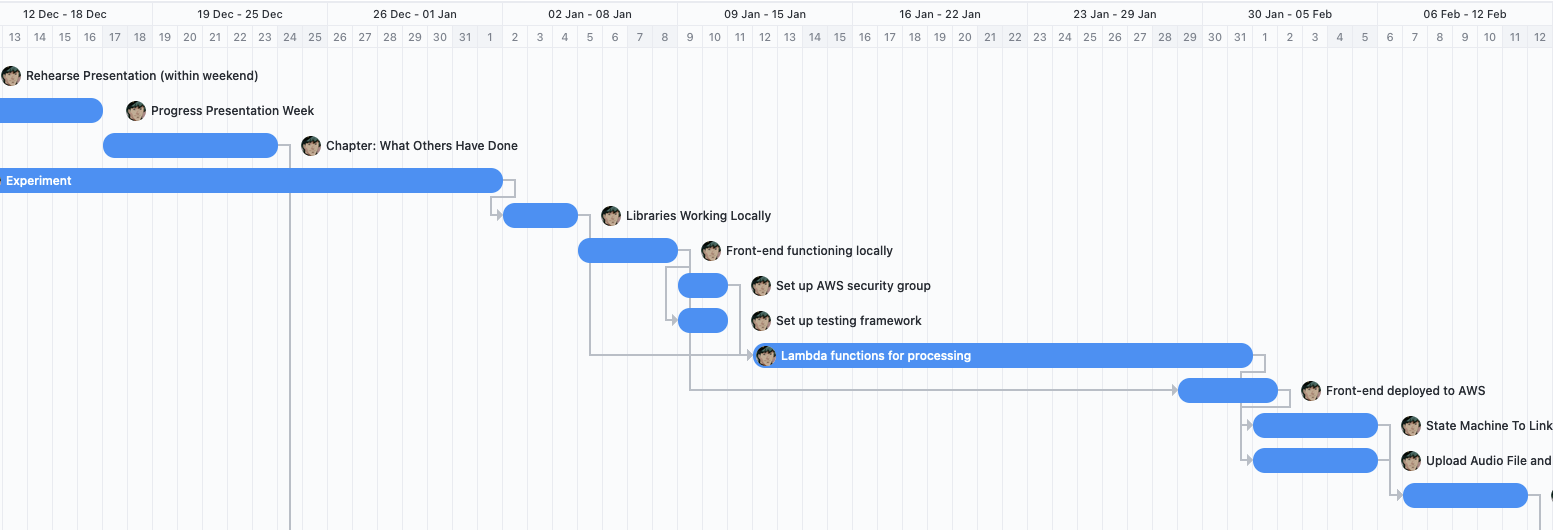
\includegraphics[width=\linewidth]{timeline1}
    \caption{Timeline: $Dec~12th~\rightarrow~Feb~12th$}\label{fig:timeline1}
    \endminipage\hfill
    \minipage{\textwidth}
    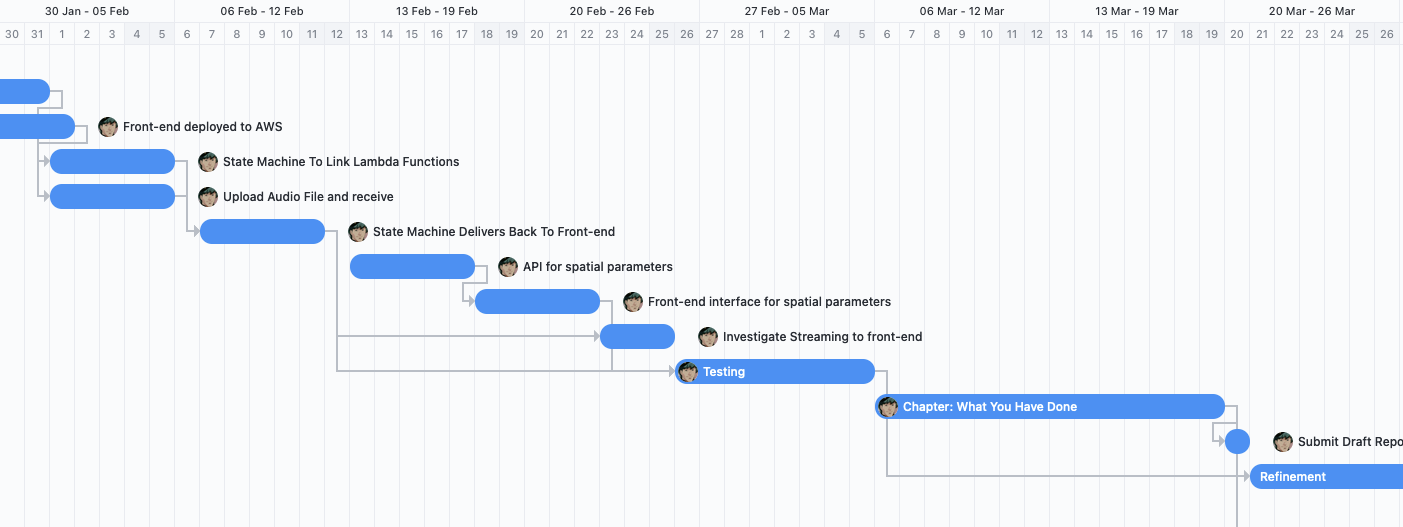
\includegraphics[width=\linewidth]{timeline2}
    \caption{Timeline: $Jan~30th~\rightarrow~Mar~26th$}\label{fig:timeline2}
    \endminipage\hfill
    \minipage{\textwidth}
    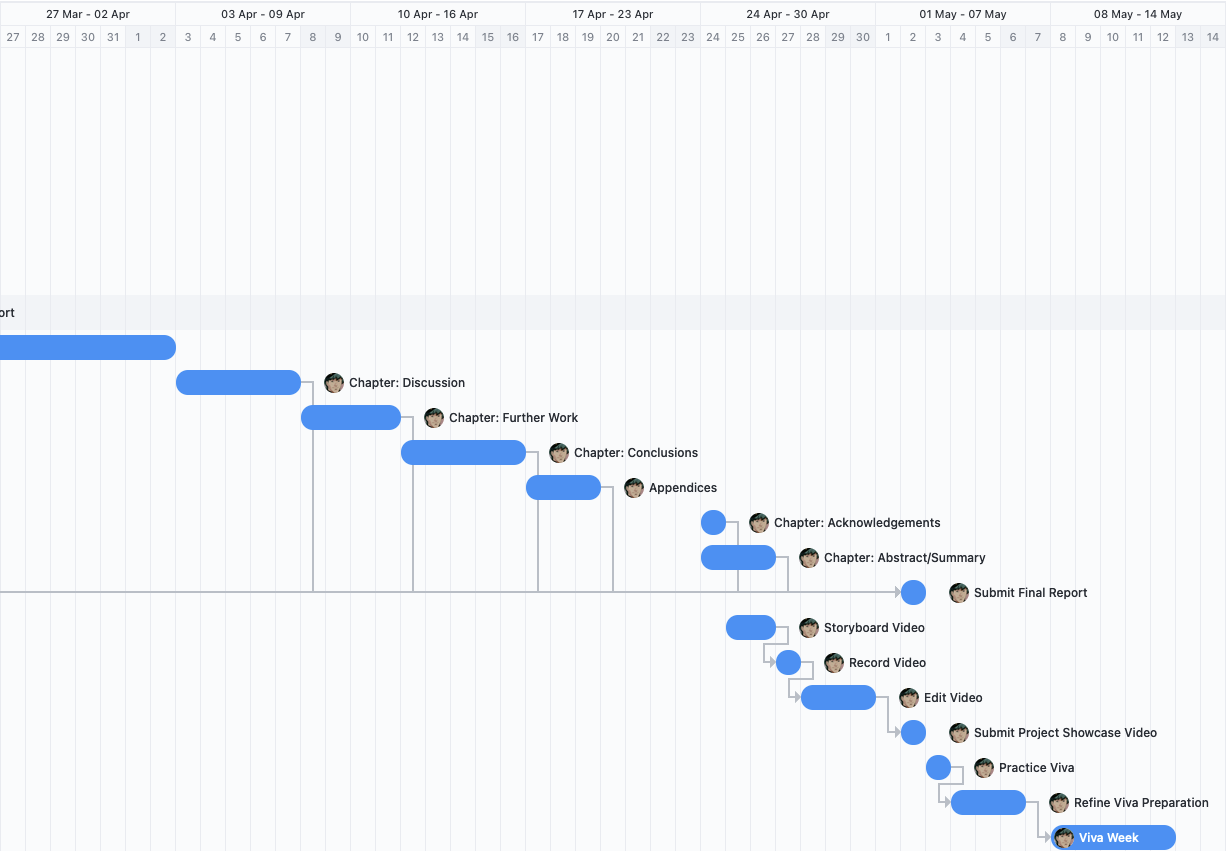
\includegraphics[width=\linewidth]{timeline3}
    \caption{Timeline: $Mar~27th~\rightarrow~May~14th$}\label{fig:timeline3}
    \endminipage
\end{figure}

\subsection{Resources}\label{subsec:resources}

This project intended to use minimal resources in its development.
As outlined in~\ref{sec:literature-review}, one of the many advantages of cloud computing is its flexibility and ease of resource management.
Given that the application would be hosted entirely in cloud environments, there would be no direct hardware costs associated with the project.
The costs that do apply will relate to the use of the~\gls{aws} platform.
These costs needed careful management, as explained in~\ref{subsec:business-risks}.

Other resources utilized included:

\begin{enumerate}
    \item Queen Mary library resources
    \item The project supervisor
    \item Knowledge sharing from colleagues at~\gls{sie}
    \item JetBrains’~\gls{ide} Suite
    \item Open-source audio-processing libraries.
    \item Online articles and tutorials
\end{enumerate}

\subsection{Methodology}\label{subsec:methodology}

\citet{murray-pm} notes that the \textquote{traditional} manner of software development follows a linear path from requirements, to design, to execution, to testing, and so on.
This method often results in inflexibility when it comes to software project execution.
This is because of its dependence on the full set of requirements being gathered before the development process begins.
Any issues with the requirements (incompleteness, inaccuracy) using this method are typically only found at the end of the process, instead of along the way through a cycle of development and feedback\footnote{\citep{murray-pm}}.
This project is of relatively small scope, and the number of shareholders are small on account of its proof-of-concept status.
As such, it serves to incorporate some, but not all, aspects of the `Agile'\footnote{\citep{beck2001agile}} development methodology into the process:

\begin{quotation}
    An Agile project starts with only the most high-level requirements.
    Sometimes these are referred to as “user stories.”
    Such a requirement might sound like, “A user will be able to buy a subscription to our product on a new e-commerce website.”
    There are no designs, no specifications.\footnote{\citep{murray-pm}}
\end{quotation}

While this project will not go so far as to remove the need for a design or specification altogether, the foundation for the project’s execution will rest on high-level user stories and identified functional requirements.
In addition, the project will require frequent testing as development progresses.
The intention, therefore, is to endeavour to implement a~\gls{cicd} pipeline to ensure any updates to the prototype can be tested and deployed in an online environment as it is being developed.

    %! Author = cspiller
%! Date = 17/11/2022

\thispagestyle{plain}
\newpage
\section{Progress Review}\label{sec:progress-review}

\normalsize
Hello\index{Hello}, world\index{world} and~\gls{aws} ~\citep{cc_overview}

%    Appendices
    \newpage
    \phantomsection
    \addcontentsline{toc}{section}{References}
    \bibliographystyle{plainnat}
    \bibliography{../../docs/src/main}

\end{document}
